\chapter{Conclusion}
\label{c:conclusion}
The Indian Summer Monsoon is one of the most influential meteorological phenomena on earth. Even though the ISM occurs every year, the exact timing and strength of its occurrence are subject to great variability and a primary factor for the welfare of the population in countries all over the Indian subcontinent. In a first part of this work, we have sought to provide insight into the strength of monsoon rainfalls by analyzing the spatial distribution of extreme rainfall events. The second part was then dedicated to the problem of predicting the timing of ISM onset over Kerala. With both of these parts, we have tried to reduce the uncertainty that is caused by the variability of ISM behavior. This chapter serves as a final conclusion to our work, with the main findings and results summarized in \cref{st:conclusion_summary} and possible extensions of our work described in \cref{st:conclusion_outlook}.

\section{Summary \& Final Conclusions}
\label{st:conclusion_summary}
Trying to provide more insight into the strength of the ISM, we have analyzed extreme monsoon rainfall using event synchronization methods and produced climate networks representing the spatial distribution of extreme rainfall events. We have then analyzed these climate networks with network measures like degree, betweenness centrality and PageRank, resulting in an intuition about the importance of locations concerning extreme rainfall. When compared to the foundational work of \citet{Stolbova.2015}, we have identified similar key regions for the pre-monsoon and monsoon seasons: while the Indian Ocean and the Tibetan Plateau are the most influential regions before the onset of the ISM, North Pakistan dominates the climate networks during the monsoon season. Our results for the post-monsoon season differ from the results in the foundational work, as the important locations in our network are concentrated over central India and the Tibetan Plateau, while the results from \citet{Stolbova.2015} primarily focus on the Tibetan Plateau.

For all of our climate network results, we have tried to link the previously described patterns to well-known phenomena that drive the yearly development of the ISM. The pre-monsoon season corresponds to the Indian summer, in which the country regularly experiences temperatures of more than 40\degree Celsius. Additionally, most rainfall is concentrated over the oceans in this season. The monsoon season is characterized by a reversal of the land-ocean temperature gradient, leading to a sea-breeze that brings moisture from the oceans onto the land. While it is non-trivial to interpret a distinct pattern like the one over North Pakistan, we proposed that the region could serve as a pivot between other key regions during this season. The final monsoon season we have analyzed, the post-monsoon season, is the season where the ISM fully withdraws from the subcontinent, and the following north-east monsoon starts to build up. We have proposed that this might cause patterns like the one seen over central India and the Tibetan Plateau.

While our first results were based mostly on the work of \citet{Stolbova.2015}, we have extended her climate network analysis by the PageRank measure as well as weighted and directed climate networks and networks thresholded at different percentiles. The PageRank of directed networks shows some new patterns when compared to the degree, as the intuition of importance is different in its ranking procedure. Further, we have found that a weighting of network edges with their synchronization coefficient makes little difference in the overall patterns and only changes minimal details. While the results of \citet{Stolbova.2015} are based on the TRMM dataset at its full resolution (0.25\degree), we have reduced the dimensionality and thus the computational requirements of the dataset by aggregating the resolution to 0.75\degree. While this could also be a reason for some of the differences in our results, they largely seem to match for two out of three seasons, with only the third season displaying bigger differences.

The second main research question in this work was the prediction of ISM onset, for which we have built prediction models based on recent neural network methods. After a long process of parameter tuning and model building, we finally got to a model architecture that manages to predict ISM onset better than comparable methods and does so from up to a one month lead. Official IMD predictions achieve a root-mean-squared error of around four days, meaning that the monsoon onset prediction can be interpreted as accurate if the real onset occurs up to four days earlier or later than the predicted date. \citet{Stolbova.2015} even counts predictions as accurate if the real onset is up to seven days early or late. In comparison, repeated evaluation of our best model yields an overall mean absolute error of 2.82 days when predicting between one and thirty days before the monsoon onset. The mentioned model tends to predict best during the week leading up to the monsoon onset, as well as more than three weeks before the onset, but performance is still good in between these periods.

Our overall best-performing model architecture takes several features of the ERA-Interim reanalysis dataset as input (mean sea-level pressure, temperature and relative humidity). Based on these inputs, a sequence of ConvLSTM and fully-connected layers manages to perform an accurate numerical prediction. On any day during the month leading up to the ISM onset, we can use our model to predict the number of days that remain until the monsoon arrives. Predictions could even be performed every day, resulting in updated predictions as more data gets available.

Even though the predictions are quite accurate, an important shortcoming in this model architecture is the practicality of the prediction approach. We trained the majority of our neural network models based on the ERA-Interim dataset, which is a meteorological reanalysis computed from both observations and simulations. The data assimilation and quality control procedures of such reanalysis datasets take their time, which is why the ERA-Interim dataset is only published with a two-month delay (not in real-time). This means that the ERA-Interim dataset cannot practically be used to predict the ISM onset, as the data for the full pre-monsoon season is only released in July. However, our architecture still can still serve as a proof that onset prediction can be performed by applying neural networks to spatiotemporal meteorological datasets and could further be used as a foundation for future models.

\newpage
\section{Future Work}
\label{st:conclusion_outlook}
The work we have presented so far could be extended in several ways, of which some would require more effort than others. In this final part of our work, we introduce the possible future extensions we could imagine and state some of our ideas for their implementation.

\paragraph{Prediction of extreme rainfall events}
The analysis of climate networks as shown in this work is only a starting point, after which a next logical step could be the prediction of extreme rainfall events. For example, one could try to predict future extreme events at a location basing on extreme events in strongly synchronous locations (that tend to lead said location).  This approach could probably only be used for short-term prediction, as the lead-time of synchronous events tends to lie within only a few days. However, even short-term predictions could potentially make a big difference concerning the safety of people affected by the predicted event.

\paragraph{Usage of different datasets}
Our final prediction model is fully focused on the ERA-Interim dataset and several of its features. While the predictions based thereon seem to be accurate and manage to outperform other comparable models, the practicality of a model based on such a reanalysis dataset is not as high as one would wish. Reanalysis datasets like ERA-Interim are only released after a certain delay (i.e., two months for ERA-Interim), which is needed for the producers to be able to perform data assimilation and quality control procedures. However, this also means that most pre-monsoon data is only fully available once the monsoon has most certainly already arrived. We suggest that the models we proposed could serve as a foundation for models that directly base on real-time datasets or purely observational datasets, and possibly multiple of them.

\paragraph{Usage of climate network results for onset prediction}
As of now, the two parts of this work, the evaluation of climate networks and the prediction of ISM onset, are strictly separate. However, a combination of the two could be imaginable, where a network measure like PageRank could be used as an additional input feature for neural network models. Such an additional feature might provide weights for the locations on the grid, which could help a neural network identify ``important'' locations that might work well as a predictor of monsoon onset.

\paragraph{Dense prediction}
Our work is solely focused on the prediction of the monsoon onset over Kerala, as it marks the arrival of monsoon on the Indian subcontinent. However, as we have described early on, an accurate estimate of monsoon arrival is of high importance for people all over India. Therefore, it would be much more useful if accurate predictions were available for all regions of India.

As a future improvement of the general applicability of our neural network models, we suggest the evaluation of an approach using ``dense prediction'' methods. Dense prediction models predict a label for each unit of the input, where a unit could be a single pixel or a region of the input image. A similar approach has been successfully applied to problems like video frame prediction, where, based on the past few frames, the next frame is to be predicted. The original work describing the ConvLSTM neural network architecture has in a sense also performed a dense prediction task, as future radar maps have been predicted based on past radar maps.

When applied to the problem of monsoon onset prediction, we could imagine that a future model would be trained to predict matrices containing the days until ISM onset for different patches of the Indian subcontinent. As we have successfully used the IMD onset dates as extracted from \citet{Singh.2009}, we would suggest a matrix with predictions based on the subregions described therein (as shown in \cref{fig:singh_subregions}). A suitable approach for handling patches of the input that are not part of any of the subregions would still need to be found, as the output dimensions of dense prediction tasks are typically equal to the input dimensions.

\begin{figure}[h!]
  \centering
  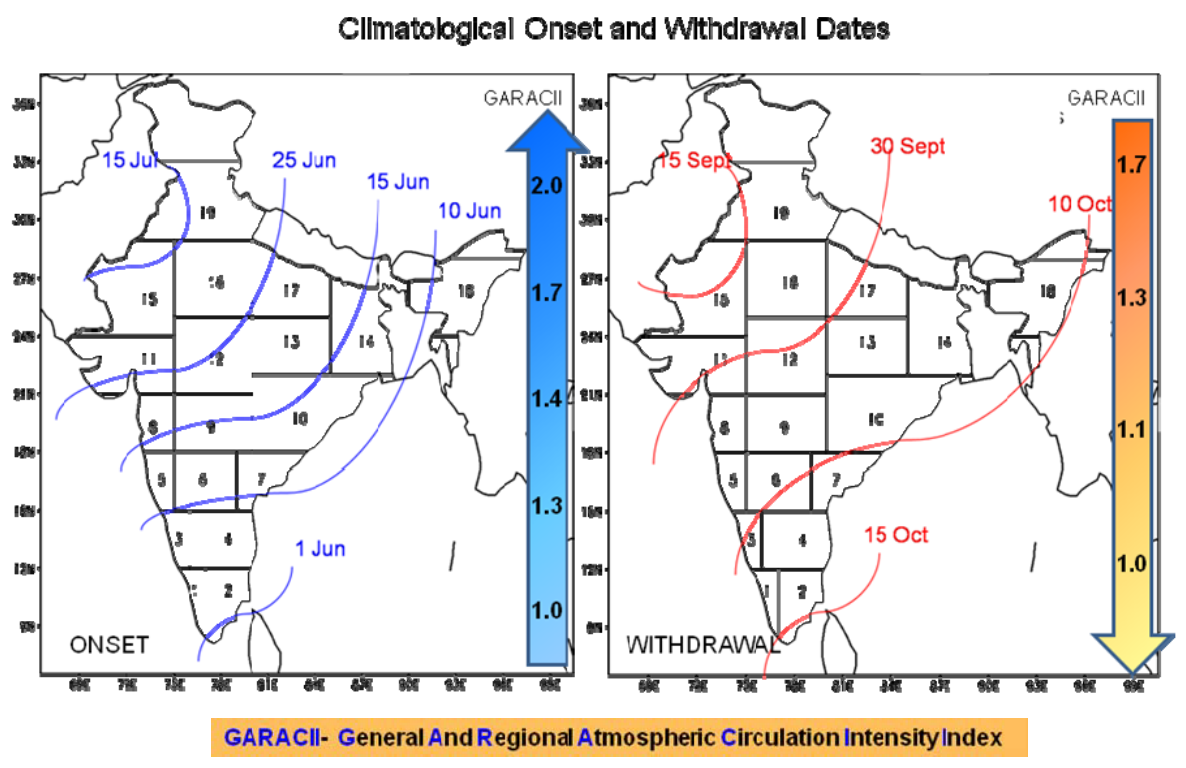
\includegraphics[width=0.6\textwidth]{./99_appendix/img/singh_subregions.png}
  \caption{Regular monsoon onset and withdrawal dates for the 19 subregions of the Indian subcontinent as depicted in \citet{Singh.2009}.}
  \label{fig:singh_subregions}
\end{figure}

\paragraph{Prediction of monsoon withdrawal}
While we have focused on predicting the monsoon onset, the withdrawal of monsoon is of similarly high importance to the Indian population, as it marks the transition from the rainy season to the winter months. Basing on our final model architecture, the withdrawal dates of the ISM could be predicted without necessitating any large changes. Using data for the monsoon season as extracted from ERA-Interim and onset dates from the IMD and \citet{Singh.2009}, a well-tuned model should be able to predict monsoon withdrawal with reasonable accuracy.
